\documentclass{jarticle}
\setlength { \textheight } { 47\baselineskip }
\setlength { \textwidth } { 50zw }
\usepackage[top=25mm, bottom=25mm, left=18mm, right=18mm]{geometry}
\usepackage{amsmath}
\usepackage{txfonts}
\usepackage{booktabs}
\usepackage{ascmac}
\usepackage{multicol}
\usepackage[dvipdfmx]{graphicx,color}
\usepackage{bm}
\usepackage{fancyhdr}
\usepackage{here}



\begin{document}

 \section*{実験の概要}
 地上には目に見えない素粒子が宇宙線として常に降り注いでいる。
 その中に存在する$\mu$粒子(ミューオン)と呼ばれる粒子の寿命を行う。
 その過程で素粒子反応、シンチレータ、光電子増陪観、論理回路、データ解析などを学ぶ。
 \section{素粒子と原子核}

  \subsection{素粒子と相互作用}
  \subsection{ファインマンダイアグラム}
  \subsection{崩壊}
  \subsection{宇宙線}
  \subsection{粒子の寿命}
  \subsection{アルミ中でのミューオン寿命}
  \subsection{核図表}
  \subsection{崩壊図}
  \section{ベータ崩壊}
  
  
  \section{ガンマ線と物質の相互作用及び測定原理}
  \subsection{コンプトン、光電効果、対生成}
  \section{確率統計}
  \section{阻止能}
  \section{シンチレータとPMTの原理}
  \subsection{シンチレータ}
	  \begin{figure}[H]
	   \begin{center}
	    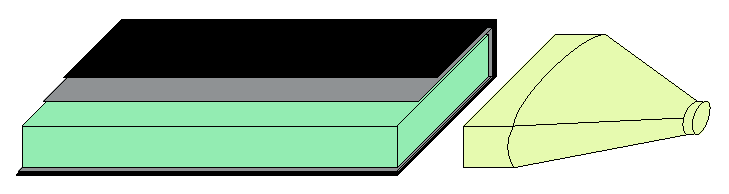
\includegraphics[width = 100mm]{./picture/Sinti.eps}
	   \end{center}
	   \caption{シンチレータとライトガイドの概略図。シンチレータはさらにマイラーと遮光材によってくるまれている。}
	   \label{Fig:Sinti}
	  \end{figure}
  
\subsection{PMT}

  \section{実習の内容}
  
  \clearpage 
  
  \section{NIM&論理回路}
  Nucelar Instrument Module(NIM) とは原子核及び素粒子実験で広く使われているモジュールシステムである。
  NIMには各モジュールに電源を供給するビン電源があり、
  各モジュールをビン電源に固定して使用する。
  
  
  \subsection{NIMモジュールとその機能}

    \subsubsection*{Discriminator}
	  
	  設定されたしきい値(threshold)よりも大きな電圧信号が入力された時、
	  設定した時間幅で決められた電圧値を出力するモジュール。
 	  
	  \begin{figure}[htbp]
	   \begin{center}
	    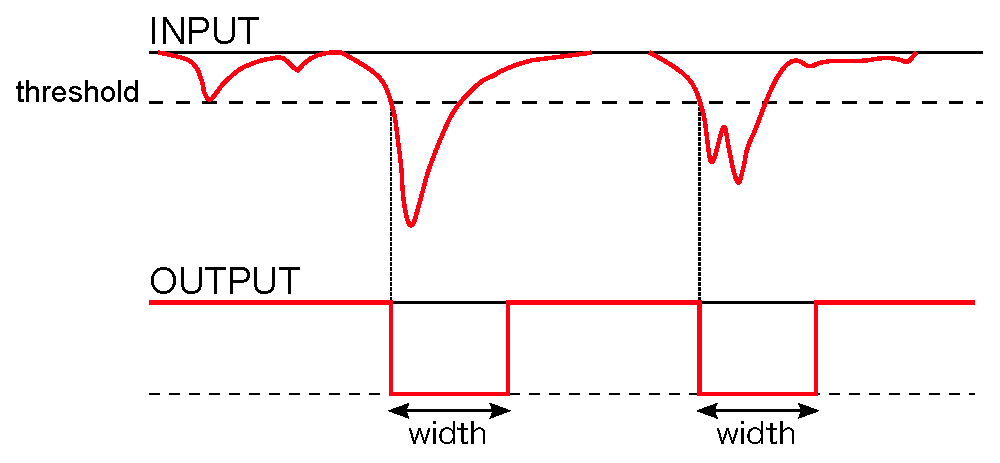
\includegraphics[width = 100mm]{./picture/Discriminator.eps}
	   \end{center}
	   \caption{Discriminatorモジュールの挙動模式図}
	   \label{Fig:Discri}
	  \end{figure}
	  
    	  \subsubsection*{Coincidence}
	  
	  2つ以上の入力ロジック信号が同時に1となった時間を起点として、
	  設定した時間幅で決められた電圧値を出力するモジュール。
	  ANDの役目を果たす。
	  
	  \begin{figure}[htbp]
	   \begin{center}
	    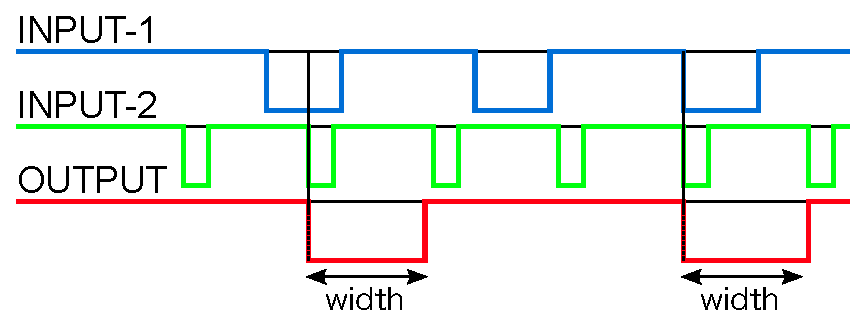
\includegraphics[width = 100mm]{./picture/Coincidence.eps}
	   \end{center}
	   \caption{Coincidenceモジュールの挙動模式図}
	   \label{Fig:Coincidence}
	  \end{figure}
	  
   \subsubsection*{FAN IN/FAN OUT}
	  
	  2つ以上の入力ロジック信号のいずれか一つでも1である間、
	  決められた電圧値を出力するモジュール
	  
	  \begin{figure}[H]
	   \begin{center}
	    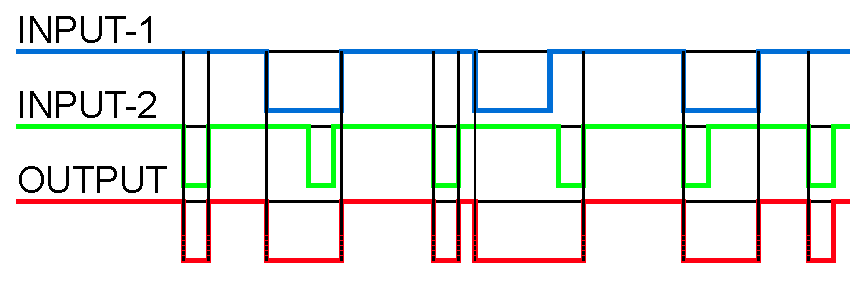
\includegraphics[width = 100mm]{./picture/FaninFanout.eps}
	   \end{center}
	   \caption{Fan-In/Fan-outモジュールの挙動模式図}
	   \label{Fig:FaninFanout}
	  \end{figure}
	  
   \subsubsection*{Delay}
    	  
    	  入力信号を設定した時間だけ遅らせて出力するモジュール。
    	  
	  \begin{figure}[H]
	   \begin{center}
	    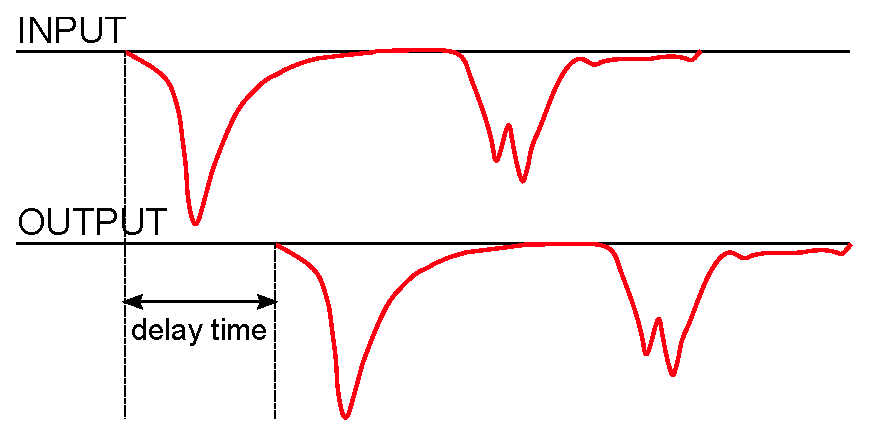
\includegraphics[width = 100mm]{./picture/Delay.eps}
	   \end{center}
	   \caption{Delayモジュールの挙動模式図}
	   \label{Fig:Delay}
	  \end{figure}
	  
	  
   \subsubsection*{Gategenerator}
   	  
	  入力ロジック信号を設定した時間だけ遅らせた後、
	  設定した時間幅だけ1の信号を出力するモジュール。
	  
	  \begin{figure}[H]
	   \begin{center}
	    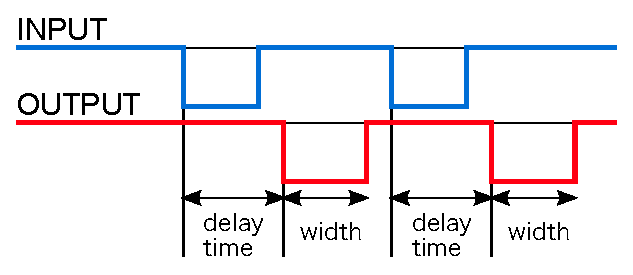
\includegraphics[width = 100mm]{./picture/Gategenerator.eps}
	   \end{center}
	   \caption{Gategeneratorモジュールの挙動模式図}
	   \label{Fig:Gategenerator}
	  \end{figure}
	  
	  
   \subsubsection*{Scaler}
	  
	  許容周波数以下の入力されたロジック信号の数を数えるモジュール。
	  
	  
	  
	  

  \subsection{CAMAC}
  Computer Automated Measurement And Control (CAMAC)

  \subsubsection*{TDC (Time to Digital Converter)}

  入力信号に遅れて停止信号を入力すると、その時間差をデータとして出力するモジュール。

	  \begin{figure}[H]
	   \begin{center}
	    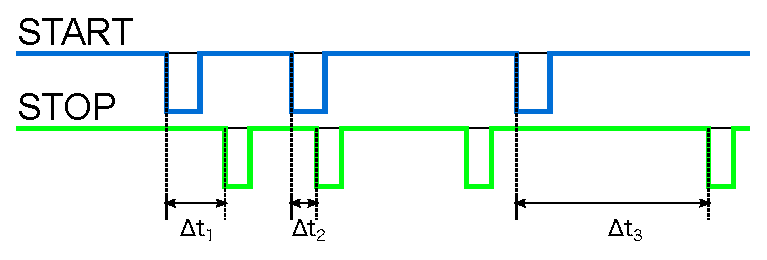
\includegraphics[width = 100mm]{./picture/TDC.eps}
	   \end{center}
	   \caption{TDCの挙動模式図。START信号が入力した後信号との時間差$\delta t_{i}$をデータとして蓄えて出力する}
	   \label{Fig:TDC}
	  \end{figure}


  
  	  \subsection{ROOT}
	  
 	  \section{実験の注意事項}
	  
 \section{データ解析の仕方と誤差}
 
 
 	  \section{実習課題}

 	  \begin{enumerate}
	   \item アナログ信号とデジタル信号の違いを信号の輸送による劣化と絡めて説明せよ。
		 
	   \item 
	  \end{enumerate}
	  
	  
	  
 \section{安全上の注意事項}
 	  \begin{enumerate}
	   \item 実験室での飲食は禁止
		 
		 特に管理区域での飲食や喫煙など、経口被爆の恐れのある行為は法律で禁止されている
		 
	   \item 放射性物質の扱いには十分注意

	   \item 放射性物質の持ち出しは禁止

	   \item 高電圧供給装置の使用前には初期値が0ボルトであることを確認すること
		 
		
	  \end{enumerate}
	  

	  
	  
	  
\clearpage

\appendix 
	  
	  
 \section{UNIX}
	  
  \subsection*{コマンドリスト}
	  

\begin{table}[htbp]
  \caption{UNIXコマンドリスト} 
  \label{Tab:UNIXコマンドリスト}
  \begin{center}
     \begin{tabular}{ll}\toprule
      カレントディレクトリを表示する &
      \verb|$ pwd | \\ \midrule
      ディレクトリを移動する &
	  \verb|$ cd| $_\sqcup$ \verb|移動先のディレクトリ | \\ \midrule
      ホームディレクトリに移動する &
	  \verb|$ cd | \\ \midrule
      ファイルの情報を表示する &
	  \verb|$ ls | \\ \midrule
      ファイルの情報を詳細に表示する &
	  \verb|$ ls| $_\sqcup$ \verb|-a| \\ \midrule
      ディレクトリを作成する &
	  \verb|$ mkdir| $_\sqcup$ \verb|作成するディレクトリ名 | \\ \midrule
      ファイルをコピーする&
	  \verb|$ cp| $_\sqcup$ \verb|コピー元ファイル名| $_\sqcup$ \verb|コピー先ファイル名 | \\ \midrule
      ファイルを移動する &
	  \verb|$ mv| $_\sqcup$ \verb| 移動元ファイル名| $_\sqcup$ \verb|移動先ディレクトリ名 | \\ \midrule
     ファイル名を変更する&
	  \verb|$ mv| $_\sqcup$ \verb|変更前ファイル名| $_\sqcup$ \verb|変更後ファイル名 | \\ \midrule
      ファイルを削除する&
	  \verb|$ rm| $_\sqcup$ \verb|ファイル名 | \\ \midrule
      空のディレクトリを削除する&
	  \verb|$ rmdir| $_\sqcup$ \verb|ディレクトリ名 | \\ \midrule
      ディレクトリを中身ごと削除する &
	  \verb|$ rm| $_\sqcup$ \verb|-r| $_\sqcup$ \verb|ディレクトリ名| \\ \midrule
      ディレクトリ以下から指定した名前の\\
      ファイルを探して表示する &
	 \verb|$ find|$_\sqcup$ \verb|ディレクトリ名| $_\sqcup$ \verb|-name| $_\sqcup$ \verb|ファイル名 | \\ \midrule
      ディレクトリ以下から指定した文字列を含む\\
      名前のファイルを探して表示する &
	 \verb|$ find|$_\sqcup$ \verb|ディレクトリ名|$_\sqcup$ \verb|-name|$_\sqcup$ \verb|'*文字列*' | \\ \midrule
      ディレクトリ以下から指定した文字列を含む\\
      ファイルを探してファイル名を表示する &
	 \verb|$ grep|$_\sqcup$ \verb|-r|$_\sqcup$ \verb|文字列|$_\sqcup$ \verb|ディレクトリ名| \\ \midrule
      ファイルをEmacsで編集する&
	  \verb|$ emacs| $_\sqcup$ \verb|ファイル名 | \\ \midrule
      ファイルをviで編集する&
	  \verb|$ vi| $_\sqcup$ \verb|ファイル名 | \\ \midrule
      ファイルを画面単位で閲覧する&
	  \verb|$ less| $_\sqcup$ \verb|ファイル名 | \\ \midrule

     \end{tabular}
  \end{center}
\end{table}



	  
\end{document}
